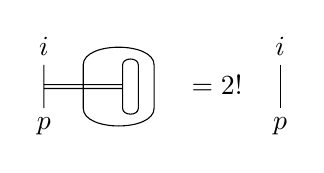
\begin{tikzpicture}
    \coordinate(origin1)at(-.5,0);
    \node at(1.7,-.255)[anchor=center]{$=2!$};
    \coordinate(origin2)at(2.5,0);
    \draw
    (origin1)node[anchor=south]{$i$}
    --++(0,-.55)node[anchor=north]{$p$}
    ++(.5,.55)node[anchor=south](j){}
    --++(0,-.55)node[anchor=north](q){}
    ++(.5,.55)node[anchor=south](k){}
    --++(0,-.55)node[anchor=north](r){}
    ++(0,.25)--++(-1,0)
    ++(0,.05)--++(1,0)
    (k.south) .. controls ++(0,.1) and ++(0,.1) .. ++(.2,0)
    --++(0,-.55)
    .. controls ++(0,-.1) and ++(0,-.1) .. (r.north)
    (j.south) .. controls ++(0,.3) and ++(0,.3) .. ++(.9,0)
    --++(0,-.55)
    .. controls ++(0,-.3) and ++(0,-.3) .. (q.north)
    ;
    \draw
    (origin2)node[anchor=south]{$i$}
    --++(0,-.55)node[anchor=north]{$p$}
    ;
\end{tikzpicture}
